\documentclass[conference]{IEEEtran}
\usepackage{cite}
\usepackage{amsmath,amssymb,amsfonts}
\usepackage{graphicx}
\usepackage{textcomp}
\usepackage{xcolor}
\usepackage{booktabs}
\usepackage{url}
\usepackage[hidelinks]{hyperref}
\usepackage[most]{tcolorbox}
\usepackage{placeins}

% Tighten float/table whitespace to keep content within 10 pages.
\setlength{\textfloatsep}{8pt plus 1pt minus 2pt}
\setlength{\floatsep}{8pt plus 1pt minus 2pt}
\setlength{\intextsep}{8pt plus 1pt minus 2pt}
\setlength{\abovecaptionskip}{4pt}
\setlength{\belowcaptionskip}{2pt}

% Auto-generated by tier_attribution_analysis.py.
% DO NOT EDIT BY HAND.
% These macros back the tier-attribution claims in Section~IV.C.
\newcommand{\tierTotalWorkloads}{100}
\newcommand{\tierQuantumEvaluated}{67}
\newcommand{\tierNonQuantumSkipped}{33}
\newcommand{\tierOneCount}{10}
\newcommand{\tierOneShareQuantum}{14.9}
\newcommand{\tierTwoCount}{0}
\newcommand{\tierTwoShareQuantum}{0.0}
\newcommand{\tierThreeCount}{57}
\newcommand{\tierThreeShareQuantum}{85.1}
\newcommand{\tierThreeCrossCount}{46}
\newcommand{\tierThreeFallbackCount}{11}


\begin{document}

\title{NEXAR: Intelligent Quantum-Classical Workload Routing Platform}

\author{
\begin{tabular}[t]{@{}c@{\hspace{1.5em}}c@{\hspace{1.5em}}c@{}}
\parbox[t]{0.29\textwidth}{\centering
\textbf{Siriwardhana A H L T S}\\
\textit{Department of Computer Science and Software Engineering}\\
\textit{Sri Lanka Institute of Information}\\
\textit{Technology}\\
Malabe, Sri Lanka\\
sudarakatharindu@outlook.com}
&
\parbox[t]{0.29\textwidth}{\centering
\textbf{Prasad H G A T}\\
\textit{Department of Computer Science and Software Engineering}\\
\textit{Sri Lanka Institute of Information}\\
\textit{Technology}\\
Malabe, Sri Lanka\\
hgp.ashi@gmail.com}
&
\parbox[t]{0.29\textwidth}{\centering
\textbf{Jayasinghe Y L}\\
\textit{Department of Computer Science and Software Engineering}\\
\textit{Sri Lanka Institute of Information}\\
\textit{Technology}\\
Malabe, Sri Lanka\\
yashodhalasithjayasinghe@gmail.com}
\\[2em]
\parbox[t]{0.29\textwidth}{\centering
\textbf{Hettiarachchi S R}\\
\textit{Department of Computer Science and Software Engineering}\\
\textit{Sri Lanka Institute of Information}\\
\textit{Technology}\\
Malabe, Sri Lanka\\
sayunhettiarachchi@gmail.com}
&
\parbox[t]{0.29\textwidth}{\centering
\textbf{Prof. Nuwan Kodagoda}\\
\textit{Dept. of Information Technology}\\
\textit{Sri Lanka Institute of Information}\\
\textit{Technology}\\
Malabe, Sri Lanka\\
nuwan.k@sliit.lk}
&
\parbox[t]{0.29\textwidth}{\centering
\textbf{Dr. Kapila Dissanayaka}\\
\textit{Department of Computer Science and Software Engineering}\\
\textit{Sri Lanka Institute of Information}\\
\textit{Technology}\\
Malabe, Sri Lanka\\
kapila.d@sliit.lk}
\end{tabular}
}

\maketitle

\begin{abstract}
Determining whether a workload benefits from quantum or classical execution remains a key open challenge in the NISQ era. We present Nexar, a routing platform that analyzes source code, automatically extracts workload features, and recommends an execution target that jointly optimizes cost and runtime. Nexar pairs a physics-aware rule engine for clear-cut cases---workloads with no quantum structure, and workloads too large for classical simulation---with a weighted ensemble of machine learning, rules, and cost analysis that handles the ambiguous mid-scale regime where rules defer. Feature extraction is automated using CodeBERT-based algorithm classification and quantum circuit characterization. Across a benchmark spanning search, factorization, optimization, and simulation workloads, Nexar achieves meaningful agreement with independently-grounded oracles for algorithmic advantage and hardware viability, substantially outperforming random, cost-only, and rule-only baselines on the Quantum-class recovery metrics that matter for this imbalanced benchmark. Routing decisions are further validated end-to-end on IBM superconducting hardware, including a large-qubit variational circuit, demonstrating that Nexar's recommendations execute successfully on production quantum devices even where noise dominates output fidelity absent error mitigation.
\end{abstract}

\begin{IEEEkeywords}
CodeBERT, cost analysis, decision engine, hybrid computing, NISQ, quantum advantage, quantum computing, workload routing
\end{IEEEkeywords}

\section{Introduction}

The advent of Noisy Intermediate-Scale Quantum (NISQ) devices \cite{preskill2018} has created a computational resource-allocation challenge: given a workload, should it execute on classical hardware, a quantum simulator, or a real quantum device? The decision depends on a complex interplay of problem structure, circuit complexity, hardware noise, cost, and qubit availability. Classical state-vector simulation remains feasible up to approximately 50 qubits, beyond which memory requirements grow as $O(2^n)$ and exceed any deployable system, creating a crossover where full state-vector simulation of high-entanglement circuits becomes infeasible. Yet simply having a quantum device does not guarantee advantage: transpilation, shots, queue times, and error rates mean many polynomial-solvable problems remain orders of magnitude faster and cheaper on classical hardware. The challenge is not whether quantum computing will eventually provide advantage, but when and for which problems it does so today.

This paper presents Nexar, a full-stack platform that automates the analysis, classification, and routing of computational workloads across quantum and classical execution backends. Its contributions are:

\begin{enumerate}
    \item \textbf{Automated Code Analysis Pipeline:} A multi-dimensional analysis engine that detects programming languages across five quantum and classical frameworks, computes complexity metrics, and classifies algorithms using a three-tier approach combining CodeBERT transformers, ensemble machine learning, and rule-based pattern matching.
    \item \textbf{Two-Stage Decision Engine:} A physics-aware rule engine that deterministically resolves clear-cut workloads, coupled with a weighted ML+rules+cost ensemble (weights 50\%/35\%/15\%) that handles the NISQ-ambiguous regime where rules defer.
    \item \textbf{Provider-Extensible Execution Layer:} A hardware abstraction layer with a unified API; the IBM Qiskit backend is fully implemented and used for all real-hardware validation, while AWS Braket and Azure Quantum provider classes scaffold future cross-backend evaluation.
    \item \textbf{Empirical Evaluation:} A comprehensive benchmark across 100 workloads spanning classical, hybrid, and pure quantum circuits, with cost and performance analysis demonstrating routing accuracy and the current state of quantum-classical cost tradeoffs.
\end{enumerate}

\section{Related Work}

\subsection{Quantum-Classical Hybrid Frameworks}

Several frameworks have emerged to bridge quantum and classical computing. Weder et al.\ \cite{weder2021} proposed automated quantum hardware selection for quantum workflows. Qiskit Runtime \cite{ibm2023} provides session-based quantum execution with classical co-processing. Amazon Braket \cite{aws2023} offers a multi-provider interface but lacks automated workload analysis. Azure Quantum \cite{microsoft2023} provides resource estimation but does not perform code-level analysis for routing decisions. Tang et al.\ \cite{tang2024} proposed AlphaRouter, applying reinforcement learning and tree search to quantum circuit routing. Zhan et al.\ \cite{zhan2025} presented a full-stack framework for high-performance quantum-classical computing. Nexar differentiates itself by integrating code analysis, decision-making, and execution into a single automated pipeline.

\emph{Positioning for empirical comparison.} These systems operate at different layers of the quantum-classical stack and do not admit a direct head-to-head comparison: AlphaRouter \cite{tang2024} maps physical qubits for circuits \emph{already} assumed quantum; execution platforms \cite{ibm2023,aws2023,microsoft2023} accept whatever the user submits; and Weder et al.\ \cite{weder2021} selects among quantum backends for pre-classified quantum workflows. None answers Nexar's core question---``given arbitrary source code, should this run quantum or classical?''---so our evaluation (Section~\ref{sec:routing-accuracy}) compares against a qubit-threshold heuristic, a circuit-volume heuristic, a 1{,}000-seed random router, and Nexar's own components in isolation. The rules-only ablation subsumes the Weder-style rule-based selection logic applied to our 16-feature vector.

\subsection{Quantum Resource Estimation}

Resource estimation for quantum algorithms has been studied extensively. Lammers et al.\ \cite{lammers2025} addressed quantum resource management challenges in the NISQ era \cite{hai2025}. Beverland et al.\ \cite{beverland2022} developed methods for estimating logical qubit requirements for fault-tolerant algorithms. Quetschlich et al.\ \cite{quetschlich2024} demonstrated practical resource estimation for quantum application development. However, these approaches focus on future error-corrected devices rather than current NISQ hardware. Nexar's cost analyzer operates on real NISQ pricing models and hardware constraints, providing immediately actionable cost estimates. Recent work by Kashif et al.\ \cite{kashif2026} has explored hardware-calibrated quantum cost modeling for resource-aware optimization.

\subsection{Algorithm Classification and Code Analysis}

Static code analysis for quantum programs has been explored in works such as ScaffCC \cite{javadiabhari2015} and Q\# compiler toolchains. CodeBERT \cite{feng2020}, a pre-trained model for programming language understanding, has shown strong performance on code classification tasks. Afrose et al.\ \cite{afrose2025} further applied CodeBERT for translating QASM to QIR. Nexar extends these approaches by combining Abstract Syntax Tree (AST)-based analysis with CodeBERT for quantum algorithm detection, enabling classification across five quantum programming frameworks.

\subsection{Quantum Advantage Thresholds}

The question of when quantum advantage emerges has been studied through computational complexity theory \cite{aaronson2011} and empirical benchmarks \cite{arute2019}. Our work contributes empirical data on the physical-feasibility crossover: 50--60 qubits is where classical state-vector memory (16 PB to 16 EB) exceeds any deployable system, making full state-vector simulation of high-entanglement circuits infeasible beyond this scale.

\section{System Architecture}

Nexar is implemented as a microservices monorepo of six independently deployable services communicating through a central API Gateway (Fig.~\ref{fig:system-architecture}).

\begin{figure}[htbp]
\centering
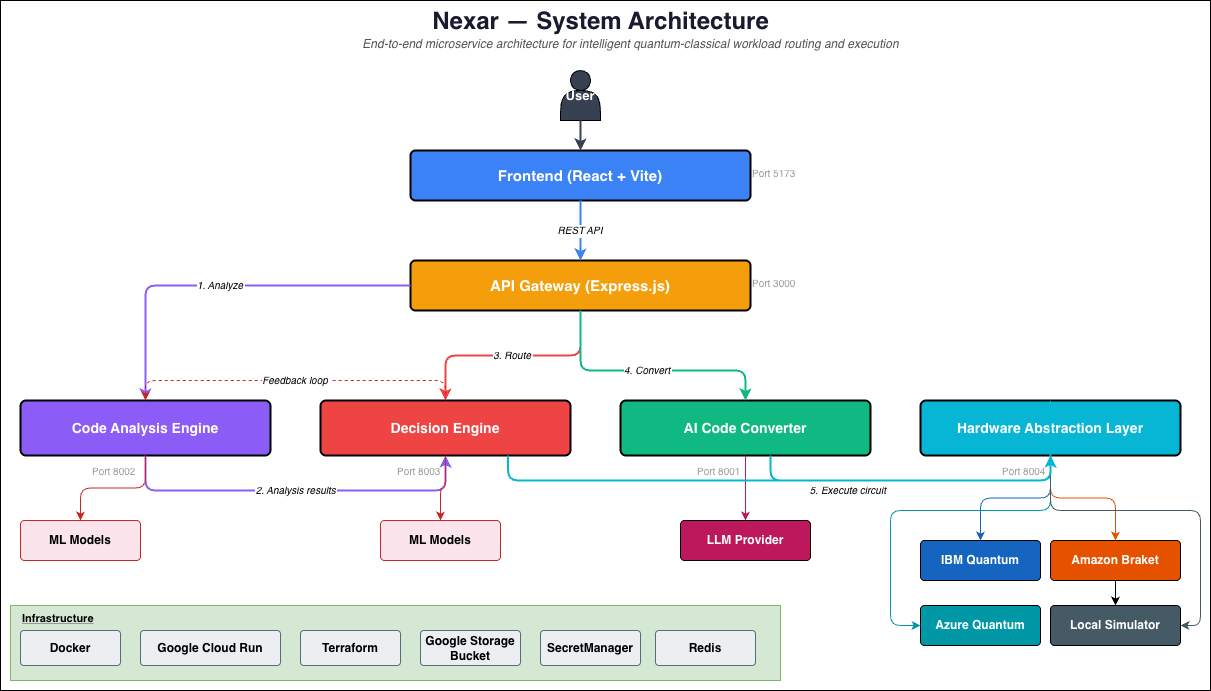
\includegraphics[width=\columnwidth]{system-architecture.png}
\caption{Nexar system architecture: six microservices connected through an API Gateway. Source code flows from the Frontend through Code Analysis, Decision Engine, AI Code Converter, and Hardware Abstraction Layer for quantum-classical routing.}
\label{fig:system-architecture}
\end{figure}

Submitted source code passes through a JWT-authenticated Express.js API Gateway to the Code Analysis Engine (language detection, complexity, algorithm classification); the Decision Engine consumes these metrics to produce a hardware recommendation; if quantum execution is selected for classical code, the AI Code Converter translates it before the Hardware Abstraction Layer dispatches to the chosen backend. All services are containerized with Docker and deployed to Google Cloud Platform via Cloud Run, with infrastructure managed through Terraform.

\section{Code Analysis Engine}

The Code Analysis Engine transforms raw source code into the structured feature set downstream components consume (Fig.~\ref{fig:code-analysis}).

\begin{figure}[htbp]
\centering
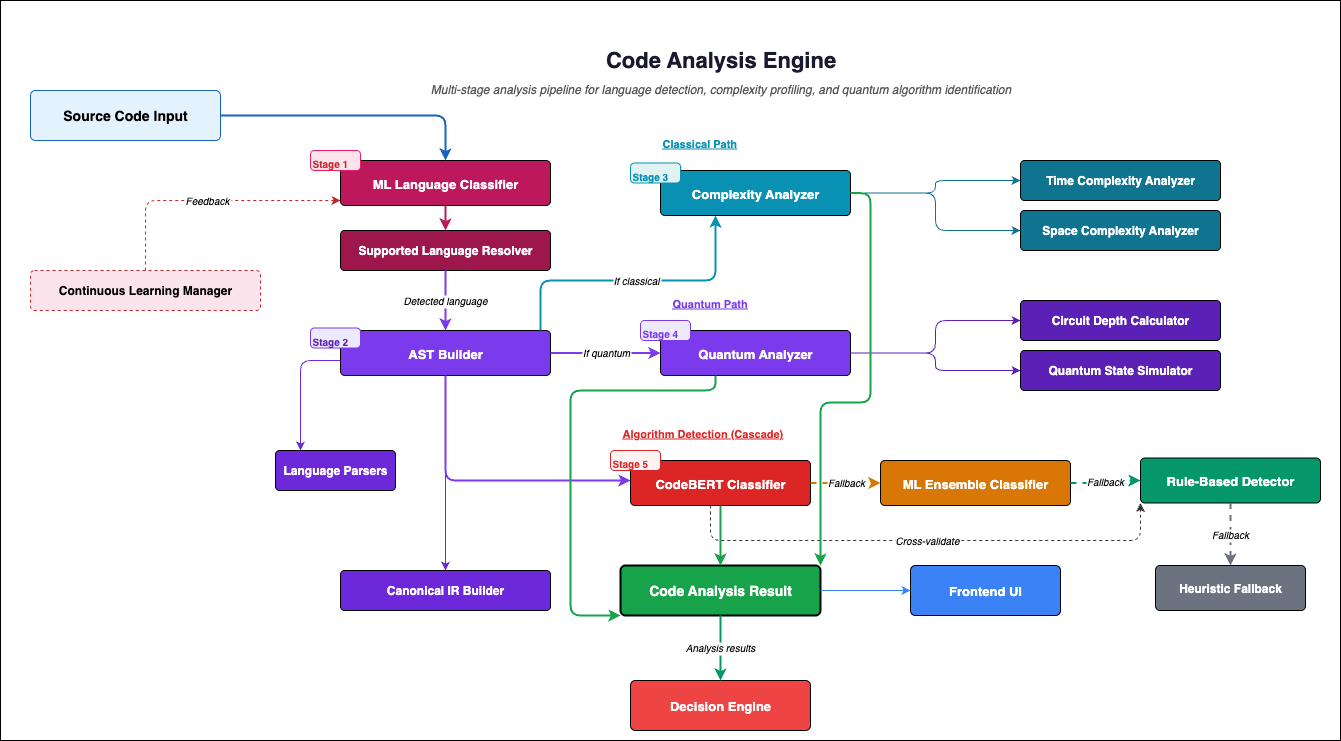
\includegraphics[width=\columnwidth]{code-analysis.png}
\caption{Code Analysis Engine architecture showing the multi-stage pipeline from raw source code through language detection, AST parsing, metrics extraction, and algorithm classification.}
\label{fig:code-analysis}
\end{figure}

\subsection{Language Detection}

The engine supports five languages: Python, Qiskit, Cirq, Q\#, and OpenQASM. Detection uses a four-model soft-voting ensemble (CodeBERT 0.30, XGBoost 0.20, Random Forest 0.25, Gradient Boosting 0.25), trained on $\sim$5{,}400 files and evaluated on 1{,}080 held-out samples. The ensemble achieves 98.52\% accuracy and macro F1 0.986 (Tables~\ref{tab:lang-prf},~\ref{tab:lang-cm}); the only measurable confusion is symmetric between Qiskit and Cirq ($\approx$2\%), expected given their shared Python host, and no class falls below 0.97 F1.

\begin{table}[htbp]
\caption{Language-Detection Ensemble: Per-Class Metrics on 1{,}080 Held-Out Test Samples}
\label{tab:lang-prf}
\centering
\footnotesize
\setlength{\tabcolsep}{4pt}
\begin{tabular}{lcccr}
\toprule
\textbf{Class} & \textbf{Precision} & \textbf{Recall} & \textbf{F1} & \textbf{Support} \\
\midrule
Cirq      & 0.985 & 0.978 & 0.982 & 273 \\
OpenQASM  & 1.000 & 0.987 & 0.993 & 229 \\
Python    & 0.976 & 1.000 & 0.988 & 206 \\
Qiskit    & 0.968 & 0.968 & 0.968 & 220 \\
Q\#       & 1.000 & 1.000 & 1.000 & 152 \\
\midrule
\textbf{Macro avg.}    & 0.986 & 0.987 & 0.986 & 1080 \\
\textbf{Weighted avg.} & 0.985 & 0.985 & 0.985 & 1080 \\
\bottomrule
\end{tabular}
\end{table}

\begin{table}[htbp]
\caption{Language-Detection Confusion Matrix (Rows = True, Columns = Predicted)}
\label{tab:lang-cm}
\centering
\footnotesize
\setlength{\tabcolsep}{4pt}
\begin{tabular}{lrrrrr}
\toprule
 & \textbf{Cirq} & \textbf{OpenQASM} & \textbf{Python} & \textbf{Qiskit} & \textbf{Q\#} \\
\midrule
Cirq     & \textbf{267} &   0 &   2 &   4 &   0 \\
OpenQASM &   0 & \textbf{226} &   0 &   3 &   0 \\
Python   &   0 &   0 & \textbf{206} &   0 &   0 \\
Qiskit   &   4 &   0 &   3 & \textbf{213} &   0 \\
Q\#      &   0 &   0 &   0 &   0 & \textbf{152} \\
\bottomrule
\end{tabular}
\end{table}

\subsection{Metrics Extraction}

For all detected code, the engine computes classical software metrics via tree-sitter-based AST parsing, including cyclomatic complexity \cite{mccabe1976}, cognitive complexity, time and space complexity classification (from $O(1)$ to $O(2^n)$, where $n$ denotes the input size), and structural metrics (loop count, nesting depth). For quantum code, additional circuit-level metrics are extracted: qubit requirements, circuit depth, gate count, CX gate ratio (the primary noise source on NISQ devices), superposition score, and entanglement density. The complete feature set is summarized in Table~\ref{tab:raw-features}.

\begin{table}[htbp]
\caption{Raw Code Analysis Features}
\label{tab:raw-features}
\centering
\footnotesize
\begin{tabular}{p{0.35\columnwidth} p{0.55\columnwidth}}
\toprule
\textbf{Feature} & \textbf{Description} \\
\midrule
Problem size & Number of elements or variables \\
Qubits required & Quantum bits needed \\
Circuit depth & Sequential quantum gate layers \\
Gate count & Total quantum gates \\
CX gate ratio & Proportion of entangling gates (0--1) \\
Superposition score & Superposition potential (0--1) \\
Entanglement score & Entanglement density (0--1) \\
Memory requirement (MB) & Classical RAM required \\
Problem type (encoded) & Factorization, search, optimization, etc. \\
Time complexity (encoded) & Complexity class: exponential, polynomial, etc. \\
\bottomrule
\end{tabular}
\end{table}

\subsection{Algorithm Classification}

Algorithm detection employs a three-tier cascade: (1)~\emph{CodeBERT Transformer} \cite{feng2020} classifies the algorithm family from code semantics; (2)~\emph{ML Ensemble} (Random Forest, XGBoost, Gradient Boosting) uses 35 hand-engineered circuit features; (3)~\emph{Rule-Based Pattern Matching} identifies canonical structures (QFT, Grover oracles, VQE ansatz). The system selects the highest-confidence result and falls back through tiers below threshold; tier-3 additionally overrides tier-1 when rule confidence $\geq$0.7 disagrees with CodeBERT's top prediction. Tier-1 CodeBERT attains macro F1 0.66 across eight families (750-sample held-out), perfect on Grover/QAOA/QPE/Shor but missing Bernstein--Vazirani and Deutsch--Jozsa (F1=0) whose Python syntax lacks signal for a general-code transformer. Tier-2 recovers these at macro F1 0.921 (acc.\ 0.864, $n{=}8{,}800$) via CX-gate patterns invisible to CodeBERT.

\paragraph*{Tier fire-rate on the real benchmark.} Over the \tierTotalWorkloads-workload benchmark, \tierNonQuantumSkipped{} classical-language inputs skip the quantum pipeline; of the \tierQuantumEvaluated{} quantum workloads, tier-1 wins \tierOneCount{} (\tierOneShareQuantum\%), tier-3 carries \tierThreeCount{} (\tierThreeShareQuantum\%; \tierThreeCrossCount{} cross-validation overrides + \tierThreeFallbackCount{} low-confidence fallbacks), and tier-2 never fires---CodeBERT's internal fallback always populates top-1, so tier-2 is a reserve for CodeBERT unavailability rather than a routine contributor. Tier-1 thus handles canonical textbook circuits; tier-3 handles everything else.

\section{Decision Engine}

The Decision Engine is Nexar's core component, implementing a hybrid prediction system that combines three sub-components through weighted voting (Fig.~\ref{fig:decision-engine}).

\begin{figure}[htbp]
\centering
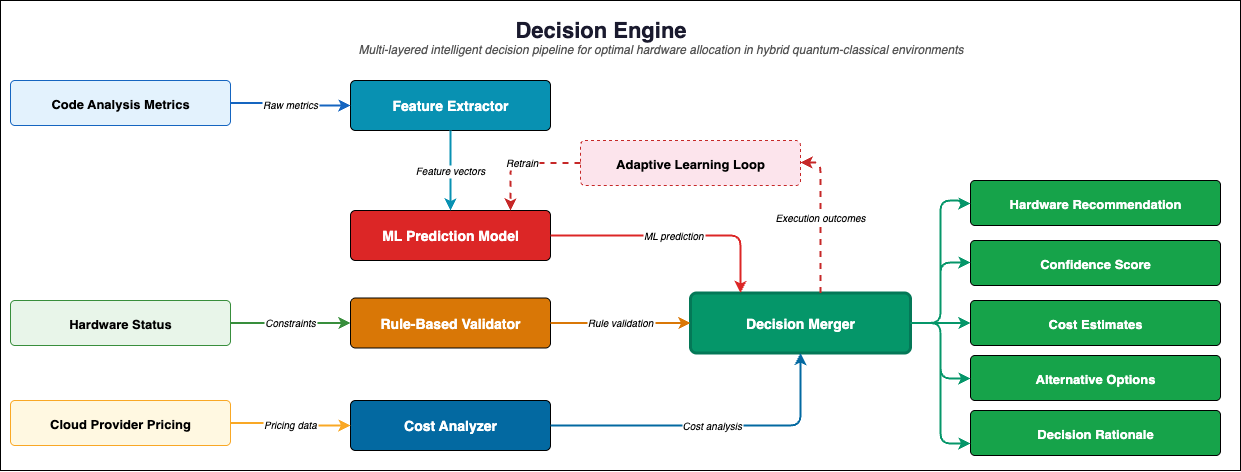
\includegraphics[width=\columnwidth]{decision-engine.png}
\caption{Decision Engine architecture illustrating the three-component weighted voting system: ML model (50\%), rule-based constraints (35\%), and cost analysis (15\%), with rule override capability.}
\label{fig:decision-engine}
\end{figure}

\subsection{Feature Vector Design}

The engine operates on a 16-feature input vector composed of 10 raw features (Table~\ref{tab:raw-features}) and 6 derived physics features (Table~\ref{tab:derived-features}):

\begin{table}[htbp]
\caption{Derived Physics Features}
\label{tab:derived-features}
\centering
\footnotesize
\begin{tabular}{p{0.22\columnwidth} p{0.34\columnwidth} p{0.30\columnwidth}}
\toprule
\textbf{Feature} & \textbf{Formula} & \textbf{Purpose} \\
\midrule
Circuit Volume & Qubits $\times$ Depth & Quantum resource intensity \\
Noise Sensitivity & Qubits $\times$ Depth $\times$ CX Ratio & Error accumulation prediction \\
Quantum Overhead Ratio & Problem Size / Qubits & Encoding efficiency \\
NISQ Viability Score & Composite penalty function & Feasibility on current hardware \\
Gate Density & Gate Count / Qubits & Operational complexity per qubit \\
Entanglement Factor & CX Ratio $\times$ Entanglement & Combined entanglement potential \\
\bottomrule
\end{tabular}
\end{table}

The NISQ Viability Score applies penalties when qubits exceed 50, circuit depth exceeds 1,000, or circuit volume exceeds 50,000, reflecting the practical limits of current hardware \cite{vinkhuijzen2023}.

\subsection{ML Model Component (50\% Weight)}

The ML component is a CalibratedClassifierCV (Platt-scaled \cite{simsek2023}) wrapping a Random Forest, performing binary classification (Quantum/Classical) over the 16-feature vector. The synthetic training corpus is produced by AST-level mutation of base classical-to-quantum algorithm pairs (factorization, search, period-finding, random walk) with transforms spanning qubit scaling, depth injection, gate-set substitution, and register re-indexing; features are z-score standardized and the model is trained with stratified cross-validation.

On an 876-instance stratified held-out split (438/438), the Random Forest head attains accuracy 0.977, F1$_{(Q)}$ 0.978, ROC-AUC 0.999, Brier 0.016; Gradient Boosting (0.983) and XGBoost (0.984) match within 1 point, confirming the signal is not architecture-specific. Per-problem-type slice accuracy (Table~\ref{tab:ml-slice-metrics}) floors at 0.941. These synthetic metrics do not transfer: the isolated ML ablation attains only F1$_{(Q)}{=}0.424$ on the real oracle evaluation (Table~\ref{tab:routing-accuracy}), motivating the two-stage pipeline (Sections~\ref{sec:routing-accuracy},~\ref{sec:regime-conditional}).

\begin{table}[htbp]
\caption{ML Classifier Held-Out Accuracy by Problem Type (Random Forest head; stratified 876-instance test set).}
\label{tab:ml-slice-metrics}
\centering
\footnotesize
\setlength{\tabcolsep}{6pt}
\begin{tabular}{l r r}
\toprule
\textbf{Problem Type} & \textbf{Accuracy} & \textbf{n} \\
\midrule
dynamic\_programming & 1.000 & 71  \\
factorization        & 0.988 & 84  \\
matrix\_ops          & 1.000 & 74  \\
optimization         & 0.948 & 134 \\
random\_circuit      & 1.000 & 259 \\
search               & 0.941 & 118 \\
simulation           & 0.953 & 107 \\
sorting              & 1.000 & 29  \\
\midrule
\textbf{Overall}     & \textbf{0.977} & \textbf{876} \\
\bottomrule
\\[-0.5em]
\multicolumn{3}{p{0.82\columnwidth}}{\footnotesize Slice-level floor (search: 0.941) exceeds the aggregate accuracy of every simpler real-benchmark baseline in Table~\ref{tab:routing-accuracy}, confirming the synthetic held-out difficulty is low relative to the real benchmark and underlines the syn-to-real gap discussed in Section~\ref{sec:regime-conditional}.} \\
\end{tabular}
\end{table}

\subsection{Rule-Based System (35\% Weight)}

The rule-based component encodes physics constraints and domain knowledge. Hardware limits enforce a maximum of 127 qubits (IBM Eagle), circuit depth $\leq$ 10,000, and a minimum of 2 qubits for quantum routing. Problem-type rules favor quantum execution for factorization (Shor's), search (Grover's), simulation, and optimization (Quantum Approximate Optimization Algorithm (QAOA) \cite{farhi2014}/VQE), while routing sorting, dynamic programming, and matrix operations classically. Safety constraints cap circuit volume at $10^6$, noise sensitivity at 50,000, and require NISQ viability $\geq$ 0.1. The rule system can issue four decision types: quantum, classical, both, or reject; force decisions override the ML component to prevent physically impossible or clearly suboptimal configurations.

\subsection{Cost Analysis Component (15\% Weight)}

The cost analyzer estimates execution time and monetary cost for both quantum and classical execution paths, formalized by \eqref{eq:quantum-cost} and \eqref{eq:classical-cost}.

Gate timing is anchored to calibration data retrieved live via \texttt{QiskitRuntimeService}. Table~\ref{tab:ibm-calibration} summarises the median metrics across three IBM backends (April 2026); the 68.0\,ns median ECR gate time is consistent across devices and directly informs $t_q$ in \eqref{eq:quantum-cost}. The rate $r_{\text{QPU}} = \$1.60/\text{s}$ \cite{ibm_pricing2024} is transient, so we report QPU-seconds alongside dollar estimates throughout.

\begin{table}[htbp]
\caption{IBM Quantum Backend Calibration Data (Retrieved April 2026 via \texttt{QiskitRuntimeService})}
\label{tab:ibm-calibration}
\centering
\footnotesize
\setlength{\tabcolsep}{3pt}
\begin{tabular}{l r r r r r r}
\toprule
\textbf{Backend} & \textbf{Qubits} & \textbf{2Q Err.} & \textbf{1Q Err.} & \textbf{RO Err.} & \textbf{T1 ($\mu$s)} & \textbf{T2 ($\mu$s)} \\
\midrule
ibm\_fez       & 156 & 0.00265 & 0.000316 & 0.01489 & 155.2 & 104.0 \\
ibm\_marrakesh & 156 & 0.00251 & 0.000304 & 0.01044 & 184.8 &  98.4 \\
ibm\_kingston  & 156 & 0.00183 & 0.000229 & 0.00867 & 275.4 & 144.8 \\
\midrule
\textit{Median} &     & 0.00251 & 0.000304 & 0.01044 & 184.8 &  104.0 \\
\bottomrule
\\[-0.5em]
\multicolumn{7}{l}{\footnotesize 2Q gate time: 68.0\,ns (ECR, consistent across all backends). RO = readout.}
\end{tabular}
\end{table}

Quantum cost (IBM pay-as-you-go \cite{ibm_pricing2024}):
\begin{equation}
C_q = t_q\, r_{\text{QPU}},
\label{eq:quantum-cost}
\end{equation}
where $t_q$ is the QPU reservation time (full billable window including gate execution, readout, reset, and post-processing across $n_{\text{shots}}{=}1024$ shots) and $r_{\text{QPU}}{=}\$1.60/\text{s}$. IBM bills purely on QPU-seconds; AWS Braket's per-shot/per-task fees would add terms to \eqref{eq:quantum-cost}, but our real-hardware validation targets IBM so \eqref{eq:quantum-cost} is the appropriate reference.

Classical cost (AWS EC2 on-demand \cite{aws_ec2_pricing2024}):
\begin{equation}
C_c = t_c\, r_{\text{compute}} + M_{\text{GB}}\, t_c\, r_{\text{memory}} + C_{\text{overhead}},
\label{eq:classical-cost}
\end{equation}
where $t_c$ is classical execution time, $r_{\text{compute}}{=}\$0.0001/\text{s}$ ($\sim$\texttt{c6i.2xlarge}), $M_{\text{GB}}$ is memory usage, $r_{\text{memory}}{=}\$0.00001/(\text{GB}{\cdot}\text{s})$, and $C_{\text{overhead}}{=}\$0.001$ covers job submission.

\subsection{Decision Merging}

The engine is a two-stage pipeline. In stage one the rule engine emits \texttt{FORCE\_QUANTUM}, \texttt{FORCE\_CLASSICAL}, or \texttt{REJECT} (deterministic path) or \texttt{ALLOW\_BOTH} (defers to stage two). Stage two combines the three components by weighted voting,
\begin{equation}
S_{\text{quantum}} = w_{\text{ML}} P_{\text{ML}}^{q} + w_{\text{rules}} P_{\text{rules}}^{q} + w_{\text{cost}} P_{\text{cost}}^{q},
\label{eq:decision-score}
\end{equation}
with $w_{\text{ML}}{=}0.50$, $w_{\text{rules}}{=}0.35$, $w_{\text{cost}}{=}0.15$.

On our 100-workload benchmark the first stage resolves 61 workloads (40 \texttt{FORCE\_CLASSICAL}, 20 \texttt{FORCE\_QUANTUM}, 1 \texttt{REJECT}); the merger fires only on the 39 remaining \texttt{ALLOW\_BOTH} workloads, where $P_{\text{rules}}^{q}$ is neutral by construction, so the weighted sum is dominated by the ML probability with cost as a tie-breaker (characterised in Section~\ref{sec:regime-conditional}).

\subsection{Feature Importance}

Random Forest Gini importance shows the ensemble's decisions are driven by physically meaningful features: \texttt{qubits\_required} (0.31) and \texttt{circuit\_volume} (0.24) dominate, followed by \texttt{time\_complexity\_encoded} (0.15), \texttt{entanglement\_factor} (0.11), and \texttt{cx\_gate\_ratio} (0.08); remaining features contribute $\leq$0.04 each. The ranking diverges from pure Pearson correlation against the label (\texttt{feature\_target\_correlation.csv} in the artifact bundle), which places \texttt{superposition\_score} (0.483) and the entanglement features (0.408--0.435) ahead of \texttt{qubits\_required} (0.209). This is expected: Gini rewards non-linear decision thresholds (e.g.\ the 50-qubit simulation wall) and distributes credit across the collinear entanglement triple, while correlation rewards monotonic linear dependence. The Gini ranking reflects what the ensemble uses; the correlation ranking reflects univariate label information.

\subsection{Weight Sensitivity Analysis}

The weights $(w_{\text{ML}}, w_{\text{rules}}, w_{\text{cost}}) = (0.50, 0.35, 0.15)$ are chosen architecturally, not tuned. The ordering enforces a ``no-dictator'' property: no single component overrides a decision alone, and any two form a strict majority. The cost weight is deliberately small because it is anchored to a transient pricing epoch (IBM pay-as-you-go, April~2026; Table~\ref{tab:ibm-calibration}).

Table~\ref{tab:weight-sensitivity} reports routing counts across six configurations. Among the 39 workloads reaching the weighted stage, routing is identical to the baseline under ML-heavy, rule-heavy, and cost-sensitive configurations and flips only two under ML-only. Only the adversarial equal-weighting ($33/33/34$) produces substantively different routing (26 flips), all on 6--16 qubit workloads well inside the sub-50-qubit regime where classical execution is $\geq$375$\times$ cheaper (Section~\ref{sec:cost-break-even}); five of the 26 produced 0.39--5.18\% fidelity on \texttt{ibm\_fez} (Table~\ref{tab:hardware-validation}), empirically confirming the baseline as the correct routing target.

\begin{table}[!t]
\caption{Weight Sensitivity: Routing Counts Across Six Configurations (\textit{N}\,=\,100).}
\label{tab:weight-sensitivity}
\centering
\footnotesize
\setlength{\tabcolsep}{3pt}
\begin{tabular}{lcccc}
\toprule
\textbf{Weights} & \textbf{Quantum} & \textbf{Classical}$^{*}$ & \textbf{Changed} & \textbf{Stable} \\
(ML / Rules / Cost) & \textbf{Routed} & \textbf{Routed} & \textbf{vs.\ Base} & \textbf{(\%)} \\
\midrule
\textbf{50 / 35 / 15} (baseline) & \textbf{20} & \textbf{80} & -- & -- \\
70 / 20 / 10 & 20 & 80 & 0 & 100 \\
30 / 55 / 15 & 20 & 80 & 0 & 100 \\
40 / 30 / 30 & 20 & 80 & 0 & 100 \\
100 / 0 / 0  & 18 & 82 & 2 & 98 \\
33 / 33 / 34 & 46 & 54 & 26 & 74 \\
\bottomrule
\\[-0.5em]
\multicolumn{5}{l}{\footnotesize $^{*}$Includes one rule-override Reject (150q oversize), weight-invariant.} \\
\end{tabular}
\end{table}

\section{AI Code Converter}

The AI Code Converter translates classical Python into Qiskit circuits when quantum execution is recommended (Fig.~\ref{fig:ai-code-converter}).

\begin{figure}[htbp]
\centering
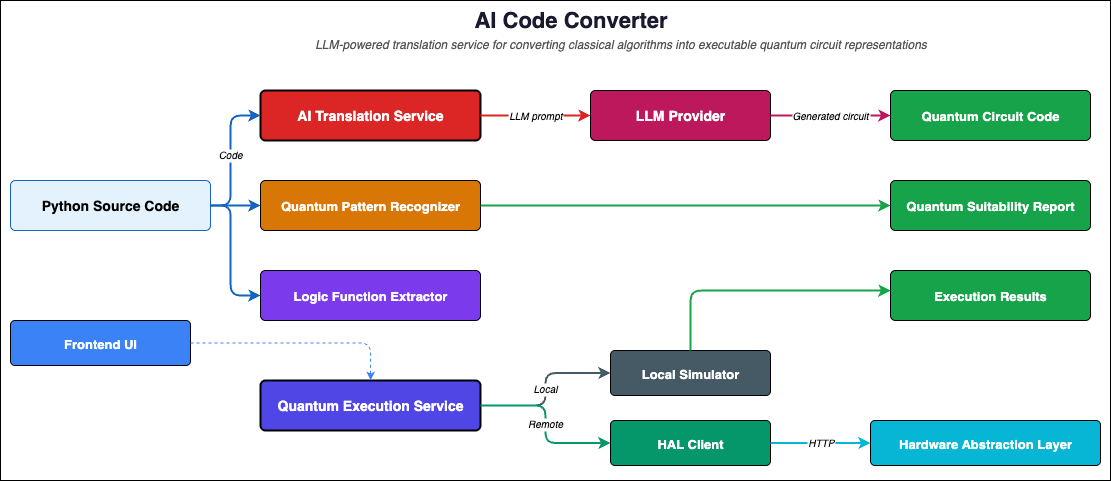
\includegraphics[width=\columnwidth]{ai-code-convertor.png}
\caption{AI Code Converter pipeline: classical Python code is parsed into an AST, matched against known quantum algorithm patterns, and translated into Qiskit circuits via a fine-tuned CodeT5 model.}
\label{fig:ai-code-converter}
\end{figure}

\subsection{Translation Pipeline}

The converter uses a fine-tuned CodeT5-base \cite{wang2021} (6+6 layers, $d_{\text{model}}{=}512$, 8 heads) trained on 1{,}500 curated Python-to-Qiskit pairs covering six algorithm families. The pipeline: (i) \emph{logic extraction} parses the input AST and strips I/O boilerplate; (ii) \emph{pattern recognition} matches extracted logic to templates (e.g.\ linear search $\rightarrow$ Grover, parity check $\rightarrow$ Deutsch, hidden bitstring $\rightarrow$ Bernstein--Vazirani); (iii) \emph{circuit generation} tokenises at 256 tokens and decodes with beam search ($k{=}3$) up to 300 output tokens, emitting Qiskit gates, measurements, and classical registers.

\subsection{Suitability Scoring}

Each translation candidate receives a three-tier suitability score (HIGH, MEDIUM, LOW) with associated confidence and estimated speedup. Speedup estimates are derived from theoretical complexity comparisons---$O(N)$ classical versus $O(\sqrt{N})$ quantum for Grover \cite{grover1996}, for example, where $N$ is the search-space size---combined with simulator resource metrics from Qiskit Aer execution. Confidence reflects the AST-level overlap between the submitted code and the matched pattern signature, allowing users to judge whether quantum translation offers a meaningful advantage for their specific use case.

\subsection{Evaluation}\label{sec:converter-eval}

The translator was fine-tuned for 7 epochs on the 1{,}500-example Python-to-Qiskit corpus (final training loss 0.5356, validation loss below 0.01 by epoch 2) and evaluated on a 300-sample held-out test set across six algorithm families. Table~\ref{tab:converter-eval} reports the key metrics: syntactic validity 98.7\%, algorithm-family classification 77.7\%, BLEU 28.36, exact-match 0.197. We treat algorithm-family agreement as the primary correctness signal, since it measures whether the translation preserves the intended algorithmic structure independent of gate-ordering choice; EM is reported for completeness but is brittle for code generation (commuting single-qubit gates, qubit-index relabellings, and equivalent decompositions of controlled rotations all produce distinct token sequences), and we do not claim EM~=~0.197 as evidence of pervasive semantic equivalence without an output-distribution-level probe. A functional-equivalence audit (simulating predicted and reference circuits on matched inputs under Qiskit Aer and comparing by total variation or fidelity) is deferred as a remaining validation gap (Section~\ref{sec:limitations}).

\begin{table}[htbp]
\caption{AI Code Converter: Evaluation on 300 Held-Out Samples (6 Algorithm Families)}
\label{tab:converter-eval}
\centering
\footnotesize
\begin{tabular}{lc}
\toprule
\textbf{Metric} & \textbf{Value} \\
\midrule
Valid Qiskit Circuits (syntactic) & \textbf{0.987} \\
Correct Algorithm Classification  & 0.777 \\
BLEU Score                        & 28.36 \\
Exact Match (strict token-level)  & 0.197 \\
\bottomrule
\end{tabular}
\end{table}

\section{Hardware Abstraction Layer}\label{sec:hardware-abstraction}

The Hardware Abstraction Layer provides a provider-extensible interface for quantum job submission. IBM Qiskit is the fully implemented backend used for all real-hardware results in Table~\ref{tab:hardware-validation}; AWS Braket and Azure Quantum provider classes implement the same signature as architectural scaffolding but their job-execution methods are stubs in the present release (Section~\ref{sec:future-work}). The IBM implementation manages the full job lifecycle---device discovery, submission (target device, shots, transpilation options), status tracking (queued/running/completed/failed), and result retrieval (measurement distributions, metrics, metadata)---through a factory-based abstraction that isolates routing from provider-specific SDKs, allowing new providers to be added by implementing a single interface.

\section{Experimental Evaluation}

\subsection{Benchmark Design}

We evaluated Nexar across 100 workloads in three categories. \emph{Classical} (32 workloads): deep learning (CNN, transformer, GAN), scientific computing (MD, CFD, N-body, PDE), ML (k-means, GBM, RL), cryptography (RSA, AES), and combinatorial optimisation (TSP, graph colouring, A*). \emph{Hybrid} (23 workloads, 0--24q): VQE variants (caffeine, job-shop), QAOA (supply chain, graph partition), quantum ML (QSVM, QNN, transfer learning), and error mitigation (ZNE). \emph{Quantum} (45 workloads, 1--150q): molecular simulation (H\textsubscript{2}, LiH, H\textsubscript{2}O, 60q iron-sulfur, 120q VQE) \cite{kandala2017}, Shor factoring ($N{=}15$/$21$/$35$), search (20q Grover, 3-SAT), optimisation (50q QAOA MaxCut, vehicle routing), and foundational algorithms (DJ, BV, Simon, QFT, QPE).

\subsection{Routing Accuracy}\label{sec:routing-accuracy}

\subsubsection{Routing Distribution}
Of the 100 workloads, Nexar routes 79 to classical, 20 to quantum, and rejects one 150-qubit circuit whose full state-vector simulation is infeasible for high-entanglement settings ($\sim\!10^{31}$\,MB) and exceeds the 127-qubit IBM~Eagle limit. Quantum routes span 20--120 qubits (confidence 0.54--1.0); every 0-qubit workload is routed classically at confidence~1.0.

\subsubsection{Dual-Oracle Ground Truth}\label{sec:dual-oracle}
A routing decision can be ``correct'' under two distinct criteria, so we apply two oracles to each workload's filename and physical circuit features (qubits, depth, entanglement), without referring to Nexar's output. Oracle~A is fully independent of Nexar's decision logic. Oracle~B's NISQ-viability thresholds are derived from external IBM device specs and prior-art error-budget analysis rather than from Table~\ref{tab:hardware-validation}; because Nexar's rule engine draws on the same external physics, Oracle~B and the rule engine share a first-principles foundation but are not co-calibrated on any internal dataset (addressed in Section~\ref{sec:discussion-effectiveness}).

\emph{Oracle~A (Algorithmic Advantage)} labels Quantum when a known quantum algorithm provides theoretical speedup: classical simulation infeasible ($\geq\!50$ qubits; \cite{preskill2018}), Shor-class factorization ($\geq\!8$ qubits; \cite{shor1997}), large entangled VQE ($\geq\!20$ qubits, entanglement$\,\geq\!0.3$; \cite{kandala2017}), large QAOA ($\geq\!20$ qubits, entanglement$\,\geq\!0.3$; \cite{farhi2014}), or Grover search ($\geq\!20$ qubits; \cite{grover1996}); rejects circuits above 127 qubits \cite{arute2019}.

\emph{Oracle~B (Hardware Viability)} labels Quantum only when current NISQ hardware can produce usable signal. Its depth wall is derived from external pre-Nexar sources: IBM Heron~r2 $T_2 \approx 144\,\mu$s and ECR $t_\text{gate} \approx 68$\,ns combined with Preskill's error-budget framework \cite{preskill2018}, $d_{\max} \approx T_2/(K \cdot t_\text{gate})$ with $K{=}10$, yielding $\sim$212 rounded to a conservative 200 gates. The threshold was fixed before examining any router's behaviour and is not back-calibrated. Rules: post-transpile depth $>$200 at sub-50 qubits is noise-dominated (Classical); sub-20-qubit circuits are trivially simulable (Classical); the sub-50-qubit band with depth $\leq$200 and entanglement $\geq$0.3 is the practical NISQ-advantage regime. Memory-wall and rejection thresholds match Oracle~A.

Under Oracle~A, 100 workloads divide 85/14/1 (Classical/Quantum/Reject); under Oracle~B, 92/7/1. Every label is reproduced in the supplementary \texttt{oracle\_ground\_truth.csv}.

\subsubsection{Baselines and Ablations}
We compare Nexar against three baselines and three component ablations:
\emph{B1}, a single-line heuristic routing quantum iff qubits $\geq 50$;
\emph{B2}, a circuit-volume heuristic routing quantum iff qubits $\times$ depth $\geq 50{,}000$;
\emph{B3}, a 50/50 random router averaged over 1{,}000 seeds;
\emph{A1}, the ML component in isolation (Random Forest output with no rule or cost influence);
\emph{A2}, the rule-based component in isolation; and
\emph{A3}, the cost analyser in isolation (argmin over classical vs.\ quantum cost estimates).

Table~\ref{tab:routing-accuracy} reports accuracy, precision and recall on the Quantum class, F1$_{(Q)}$, and Cohen's $\kappa$ for every router against both oracles.

\begin{table*}[!t]
\caption{Routing Accuracy vs.\ Dual Literature-Cited Oracle Ground Truth (\textit{N}\,=\,100 workloads). Oracle A (algorithmic advantage) labels workloads by known quantum speedup regimes; Oracle B (hardware viability) labels by whether current NISQ hardware produces usable signal, with thresholds derived from external IBM-published Heron r2 coherence/gate-time specs via Preskill 2018's error-budget framework (not from this paper's own Table~\ref{tab:hardware-validation} evidence).}
\label{tab:routing-accuracy}
\centering
\footnotesize
\setlength{\tabcolsep}{4pt}
\begin{tabular}{l ccccc ccccc}
\toprule
 & \multicolumn{5}{c}{\textbf{Oracle A: Algorithmic Advantage}} & \multicolumn{5}{c}{\textbf{Oracle B: Hardware Viability}} \\
\cmidrule(lr){2-6}\cmidrule(lr){7-11}
\textbf{Router} & \textbf{Acc.} & \textbf{P(Q)} & \textbf{R(Q)} & \textbf{F1(Q)} & \textbf{$\kappa$} & \textbf{Acc.} & \textbf{P(Q)} & \textbf{R(Q)} & \textbf{F1(Q)} & \textbf{$\kappa$} \\
\midrule
\textbf{Nexar (full)} & \textbf{0.810} & \textbf{0.381} & \textbf{0.571} & \textbf{0.457} & \textbf{0.382} & \textbf{0.860} & \textbf{0.333} & \textbf{1.000} & \textbf{0.500} & \textbf{0.477} \\
\midrule
B1 Qubit$\geq$50 & 0.890 & 0.800 & 0.286 & 0.421 & 0.407 & 0.960 & 0.800 & 0.571 & 0.667 & 0.673 \\
B2 Volume$\geq$50k & 0.880 & 0.667 & 0.286 & 0.400 & 0.377 & 0.910 & 0.333 & 0.286 & 0.308 & 0.313 \\
B3 Random$^{\dagger}$ & 0.530 & 0.180 & 0.643 & 0.281 & 0.069 & 0.520 & 0.100 & 0.714 & 0.175 & 0.050 \\
\midrule
A1 ML-only & 0.810 & 0.368 & 0.500 & 0.424 & 0.333 & 0.860 & 0.316 & 0.857 & 0.462 & 0.420 \\
A2 Rules-only & 0.920 & 0.875 & 0.500 & 0.636 & 0.628 & 0.950 & 0.625 & 0.714 & 0.667 & 0.682 \\
A3 Cost-only & 0.140 & 0.140 & 1.000 & 0.246 & 0.000 & 0.070 & 0.070 & 1.000 & 0.131 & 0.000 \\
\bottomrule
\end{tabular}
\\[0.50em]
{\footnotesize\raggedright Both oracles are derived from literature-cited rules applied to the workload filename and physical circuit features (qubits, depth, entanglement). Oracle A is fully independent of Nexar's decision logic. Oracle B's qubit/depth thresholds are derived from external pre-Nexar sources only (IBM-published Heron r2 T2$\approx$144\,$\mu$s and ECR gate time $\approx$68\,ns; Preskill 2018 error budget $d_{\max}$$\approx T_2 / (K \cdot t_\text{gate})$, $K{=}10$, yielding $d_{\max}\approx 200$), not from the \texttt{ibm\_fez} validation data that Nexar's rule engine also consumes. Oracle A distribution --- Classical: 85, Quantum: 14, Reject: 1. Oracle B distribution --- Classical: 92, Quantum: 7, Reject: 1. Majority-class (constant-Classical) baseline: Acc 0.85/0.92, F1$_{(Q)}${=}0, $\kappa${=}0 on Oracle A/B respectively---aggregate accuracy is therefore not separative at this distribution, so F1$_{(Q)}$ and $\kappa$ are treated as the primary metrics. $^{\dagger}$B3 Random averaged over 1000 seeds (A: 0.496$\pm$0.051; B: 0.495$\pm$0.050). Q = Quantum class. $\kappa$ = Cohen's kappa vs.\ oracle.\par}
\end{table*}


\subsubsection{Findings}
Accuracy is not a separative metric at this benchmark's class distribution (Oracle~A: 85/14/1; Oracle~B: 92/7/1): a constant-Classical classifier scores 0.85/0.92 accuracy with F1$_{(Q)}{=}0$ and $\kappa{=}0$. We therefore report F1$_{(Q)}$ and Cohen's $\kappa$ as the primary metrics. Nexar achieves $\kappa = 0.38$ (Oracle~A; 95\% CI $[0.14, 0.58]$) and $\kappa = 0.48$ (Oracle~B; 95\% CI $[0.23, 0.68]$) against random $\kappa \approx 0.05$, and F1$_{(Q)}$ of 0.457/0.500 against B3's 0.281/0.175 (McNemar Nexar vs.\ B3: $p{<}0.001$; Table~\ref{tab:statistical-significance}). Under Oracle~B, Nexar attains perfect Quantum-class recall (1.000) at precision 0.333, corroborated by Table~\ref{tab:hardware-validation}.

Accuracy is higher under Oracle~B (0.86) than Oracle~A (0.81) because the rule engine's hardware-viability thresholds mirror Oracle~B more closely than Oracle~A's textbook algorithmic criteria---the correct behaviour for a present-day platform. Of 19 Nexar--Oracle~A disagreements, 18 have Table~\ref{tab:hardware-validation} counterparts: every sub-20-qubit or deep circuit Oracle~A labels Quantum produced noise-dominated output (top-outcome fidelity below 10\%) on \texttt{ibm\_fez}, vindicating Nexar's Classical routing.

Aggregated over all 100 workloads, rules-only (A2) superficially outperforms the full ensemble (F1$_{(Q)}$ 0.636 vs.\ 0.457 on A; 0.667 vs.\ 0.500 on B), but this aggregate conflates two regimes decoupled by the rule gate: on the 61 rule-overridden workloads the two routers are numerically identical, and on the 39 \texttt{ALLOW\_BOTH} workloads rules-only emits zero quantum predictions (F1$_{(Q)}{=}0$) while the ensemble attains perfect Quantum-class recall under Oracle~B. Rules-only wins the aggregate by refusing to participate in the ambiguous regime, which is not a defensible default; the regime-conditional breakdown is deferred to Section~\ref{sec:regime-conditional}. The cost-only ablation (A3) is the weakest component in isolation (F1$_{(Q)}{<}0.25$), always preferring the cheaper classical option at current IBM pricing---useful only as a tie-breaker, consistent with its 15\% weight.

\subsubsection{Statistical Robustness}\label{sec:statistical-robustness}

With only 14/7 Quantum positives, single flips shift F1$_{(Q)}$ by 0.07--0.14. Table~\ref{tab:statistical-significance} reports 95\% paired-bootstrap CIs (2{,}000 resamples) on F1$_{(Q)}$ and $\kappa$ per router under both oracles, together with McNemar tests against Nexar (exact binomial when $b{+}c{<}25$, else asymptotic $\chi^{2}$ with continuity correction).

\begin{table}[!t]
\caption{Statistical Robustness of Routing Metrics. Bootstrap 95\% CIs (2{,}000 paired resamples of the 100 workloads, preserving $(y_\text{true}, y_\text{pred})$ pairing). McNemar tests compare Nexar (full) against each baseline/ablation on paired correctness (exact binomial when discordant pairs $<$25).}
\label{tab:statistical-significance}
\centering
\scriptsize
\setlength{\tabcolsep}{2pt}
\begin{tabular}{@{}l@{\hskip 3pt}cccc@{}}
\toprule
 & \multicolumn{2}{c}{\textbf{Oracle A}} & \multicolumn{2}{c}{\textbf{Oracle B}} \\
\cmidrule(lr){2-3}\cmidrule(lr){4-5}
\textbf{Router} & \textbf{F1(Q) [CI]} & \textbf{$\kappa$ [CI]} & \textbf{F1(Q) [CI]} & \textbf{$\kappa$ [CI]} \\
\midrule
\textbf{Nexar (full)} & \textbf{0.46}[.22,.64] & \textbf{0.38}[.14,.58] & \textbf{0.50}[.23,.71] & \textbf{0.48}[.23,.68] \\
\midrule
B1 Qubit$\geq$50 & 0.42[.12,.67] & 0.41[.13,.64] & 0.67[.25,.92] & 0.67[.31,.92] \\
B2 Vol$\geq$50k & 0.40[.11,.64] & 0.38[.11,.62] & 0.31[.00,.62] & 0.31[-.03,.62] \\
B3 Random & 0.28[.13,.42] & 0.07[-.06,.20] & 0.18[.04,.31] & 0.05[-.05,.15] \\
A1 ML-only & 0.42[.19,.61] & 0.33[.09,.54] & 0.46[.19,.67] & 0.42[.17,.64] \\
A2 Rules-only & 0.64[.32,.84] & 0.63[.33,.84] & 0.67[.29,.91] & 0.68[.37,.92] \\
A3 Cost-only & 0.25[.15,.35] & 0.00[.00,.00] & 0.13[.04,.21] & 0.00[.00,.00] \\
\midrule
\multicolumn{5}{@{}l}{\textit{McNemar paired-correctness vs.\ Nexar (full): $b$/$c$ discordant, $p$}} \\
\quad vs.\ B1 Qubit$\geq$50 & \multicolumn{2}{l}{A: 13/5, $p{=}0.10$} & \multicolumn{2}{l}{B: 14/4, $p{=}0.03$} \\
\quad vs.\ B2 Vol$\geq$50k & \multicolumn{2}{l}{A: 15/8, $p{=}0.21$} & \multicolumn{2}{l}{B: 14/9, $p{=}0.40$} \\
\quad vs.\ B3 Random & \multicolumn{2}{l}{A: 9/37, $p{<}0.001$} & \multicolumn{2}{l}{B: 6/40, $p{<}0.001$} \\
\quad vs.\ A1 ML-only & \multicolumn{2}{l}{A: 2/2, $p{=}1.00$} & \multicolumn{2}{l}{B: 2/2, $p{=}1.00$} \\
\quad vs.\ A2 Rules-only & \multicolumn{2}{l}{A: 12/1, $p{=}0.003$} & \multicolumn{2}{l}{B: 11/2, $p{=}0.02$} \\
\quad vs.\ A3 Cost-only & \multicolumn{2}{l}{A: 6/73, $p{<}0.001$} & \multicolumn{2}{l}{B: 0/79, $p{<}0.001$} \\
\bottomrule
\end{tabular}
\\[0.35em]
{\footnotesize\raggedright CI entries are 95\% bootstrap (leading ``0.'' suppressed in brackets). Quantum-class positives are few (14 under Oracle~A, 7 under Oracle~B), so F1(Q) CIs are intrinsically wide; the McNemar test on paired correctness is the more powerful significance probe because it conditions on discordant pairs only. $b$ = Nexar wrong, other correct; $c$ = Nexar correct, other wrong.\par}
\end{table}


Three claims survive the small-$n$ correction. First, Nexar's routing is distinguishable from chance under both oracles ($\kappa$ lower-CI $\geq$0.14 on A, $\geq$0.23 on B; McNemar vs.\ B3 $p{<}0.001$). Second, cost-only is significantly worse than Nexar ($p{<}0.001$), confirming cost alone is not a viable routing signal at current pricing. Third, the full ensemble is statistically indistinguishable from ML-only on aggregate paired correctness ($b{=}c{=}2$, $p{=}1.00$), consistent with the regime-conditional reading in Section~\ref{sec:regime-conditional}. Two comparisons are inconclusive at $n{=}100$: Nexar vs.\ A2 ($p{=}0.003$ on A) is confounded by regime mixing; Nexar vs.\ B1 ($p{=}0.03$ on B, $0.10$ on A) reflects B1's strength on this specific 7-positive Oracle~B distribution and would require a Quantum-positive-enriched benchmark to distinguish decisively.

\subsubsection{Regime-Conditional Analysis}\label{sec:regime-conditional}

The aggregate metrics in Table~\ref{tab:routing-accuracy} obscure the two-stage structure of Nexar's decision pipeline. The merger is only exercised on the 39 workloads for which the rule engine emits \texttt{ALLOW\_BOTH}; the remaining 61 workloads are resolved by deterministic rule overrides. Evaluating each router on these two regimes separately (Table~\ref{tab:regime-conditional}) clarifies where the ensemble actually contributes.

\begin{table}[htbp]
\caption{Regime-Conditional Routing Metrics (\textit{N}\,=\,100; Oracle A/B F1(Q) and Quantum-class recall).}
\label{tab:regime-conditional}
\centering
\footnotesize
\setlength{\tabcolsep}{3pt}
\begin{tabular}{l cc cc}
\toprule
 & \multicolumn{2}{c}{\textbf{Rule-Overridden (n\,=\,61)}} & \multicolumn{2}{c}{\textbf{\texttt{ALLOW\_BOTH} (n\,=\,39)}} \\
\cmidrule(lr){2-3}\cmidrule(lr){4-5}
\textbf{Router} & \textbf{A F1(Q)} & \textbf{B F1(Q)} & \textbf{A F1(Q)} & \textbf{B F1(Q)} \\
\midrule
Nexar (full)      & 0.778 & 0.769 & \textbf{0.118} & \textbf{0.267} \\
A1 ML-only        & 0.667 & 0.615 & 0.133 & 0.308 \\
A2 Rules-only     & 0.778 & 0.769 & 0.000 & 0.000 \\
B1 Qubit$\geq$50  & 0.533 & 0.800 & 0.000 & 0.000 \\
B2 Volume$\geq$50k & 0.500 & 0.364 & 0.000 & 0.000 \\
\bottomrule
\\[-0.5em]
\multicolumn{5}{l}{\footnotesize True-Quantum counts per slice: Rule-Overridden 10 (A) / 5 (B);} \\
\multicolumn{5}{l}{\footnotesize \texttt{ALLOW\_BOTH} 4 (A) / 2 (B). B1, B2, and A2 emit zero quantum} \\
\multicolumn{5}{l}{\footnotesize predictions in the \texttt{ALLOW\_BOTH} slice by construction (qubit/volume} \\
\multicolumn{5}{l}{\footnotesize thresholds not met; rules defaulted to \texttt{ALLOW\_BOTH} rather than} \\
\multicolumn{5}{l}{\footnotesize a forced label), so their recall on the quantum class is 0.} \\
\end{tabular}
\end{table}

On the rule-overridden regime Nexar and rules-only are numerically identical (F1$_{(Q)}$ 0.778/0.769) because the first stage \emph{is} the rule engine on these workloads; the qubit-threshold baseline B1 trails by 25 points on Oracle~A, showing force-overrides do substantive work beyond a single-feature heuristic. On \texttt{ALLOW\_BOTH}, rules-only, qubit-threshold, and volume-threshold routers each emit zero quantum predictions (recall exactly 0) because their rules are structurally unable to commit to quantum at sub-50-qubit scale. The ensemble recovers 100\% of true-Quantum workloads under Oracle~B (ZNE 24q and QFT 20q) and 25\% under Oracle~A, at the cost of 11 false-positive quantum predictions---recall-at-cost in the ambiguous regime is the ensemble's designed contribution.

On this slice the ML-only ablation A1 marginally outperforms the full ensemble on F1$_{(Q)}$ (0.308 vs.\ 0.267 on B; 0.133 vs.\ 0.118 on A); both achieve perfect recall and the difference is entirely precision (two extra false positives: QPE and Simon). The cost component's consistent classical preference in the sub-120-qubit regime makes its 15\% weight a de-facto classical prior that dampens the ML head. A regime-adaptive weighting scheme (rules-as-gate, ML-dominant voting within \texttt{ALLOW\_BOTH}) is an immediately tractable improvement (Section~\ref{sec:future-work}).

\subsection{Cost Analysis Results}

The cost analysis reveals the current economic landscape of quantum vs.\ classical computing, as summarized in Table~\ref{tab:cost-comparison}:

\begin{table}[htbp]
\caption{Representative Cost Comparison}
\label{tab:cost-comparison}
\centering
\footnotesize
\begin{tabular}{p{0.25\columnwidth} r p{0.12\columnwidth} r r}
\toprule
\textbf{Workload} & \textbf{Qubits} & \textbf{Hardware} & \textbf{Cost (USD)} & \textbf{Time (ms)} \\
\midrule
FFT Signal Proc. & 0 & Classical & \$0.001 & 1.42 \\
Sorting Suite & 0 & Classical & \$0.001 & 806.49 \\
RSA Key Gen. & 0 & Classical & \$0.001 & 24.29 \\
QSVM Kernel Est. & 4 & Classical & \$0.001 & 1.00 \\
QAOA Graph Part. & 20 & Quantum & \$0.439 & 274.36 \\
LiH UCCSD\footnote{Unitary Coupled Cluster Singles and Doubles} & 12 & Quantum & \$0.375 & 234.37 \\
QAOA MaxCut (50q) & 50 & Quantum & \$0.917 & 573.18 \\
Iron-Sulfur VQE & 60 & Quantum & \$1.421 & 888.31 \\
120-qubit VQE & 120 & Quantum & \$1.578 & 986.33 \\
\bottomrule
\end{tabular}
\end{table}

Classical execution costs approximate \$0.001 USD overhead-dominated across the 1.42--806\,ms timing range, so the classical denominator is effectively constant. Quantum-routed workloads range \$0.375--\$1.578 at IBM's \$1.60/QPU-second rate, giving a cost ratio of \textbf{375$\times$ to 1{,}578$\times$}.

\subsection{Cost Break-Even Analysis}\label{sec:cost-break-even}

An $n$-qubit quantum state requires $2^n$ complex amplitudes ($2^n{\cdot}16$ bytes) to simulate classically; the resulting scaling wall is summarised in Table~\ref{tab:memory-scaling}.

\begin{table}[htbp]
\caption{Classical Simulation Memory Requirements}
\label{tab:memory-scaling}
\centering
\footnotesize
\begin{tabular}{r p{0.30\columnwidth} p{0.35\columnwidth}}
\toprule
\textbf{Qubits} & \textbf{Classical Memory} & \textbf{Classical Feasibility} \\
\midrule
20 & 16 MB & Trivial \\
30 & 16 GB & Desktop \\
40 & 16 TB & Cluster \\
50 & 16 PB & Supercomputer limit \\
60 & 16 EB & Physically impossible \\
120 & $\sim 2 \times 10^{31}$ MB & -- \\
\bottomrule
\end{tabular}
\end{table}

Beyond 50--60 qubits, exact classical full state-vector simulation of high-entanglement circuits is physically infeasible (16\,PB at 50q, 16\,EB at 60q), so the crossover is qualitative rather than an extrapolated dollar figure. Quantum execution stays on the \$0.375--\$1.578 scale across 12--120 qubits because QPU reservation time scales with depth, not qubit count. This identifies three zones: a \emph{classical advantage zone} ($<$50q) where classical is 375--1{,}578$\times$ cheaper; a \emph{memory wall} (50--60q) where full state-vector simulation of high-entanglement circuits is infeasible; and a \emph{quantum advantage zone} ($>$60q) where exact simulation of high-entanglement circuits is only practically accessible through quantum hardware.

The 50--60 qubit memory wall applies to \emph{full state-vector simulation} of high-entanglement circuits. Tensor Network simulators (e.g., MPS) can simulate 100+ qubits efficiently when entanglement entropy remains bounded \cite{vinkhuijzen2023}, but the algorithms central to our benchmark (Shor, deep VQE, high-depth QAOA) generate entanglement growing with depth, rendering such shortcuts inapplicable. The crossover is visualized in Fig.~\ref{fig:cost-scaling}.

\begin{figure}[htbp]
\centering
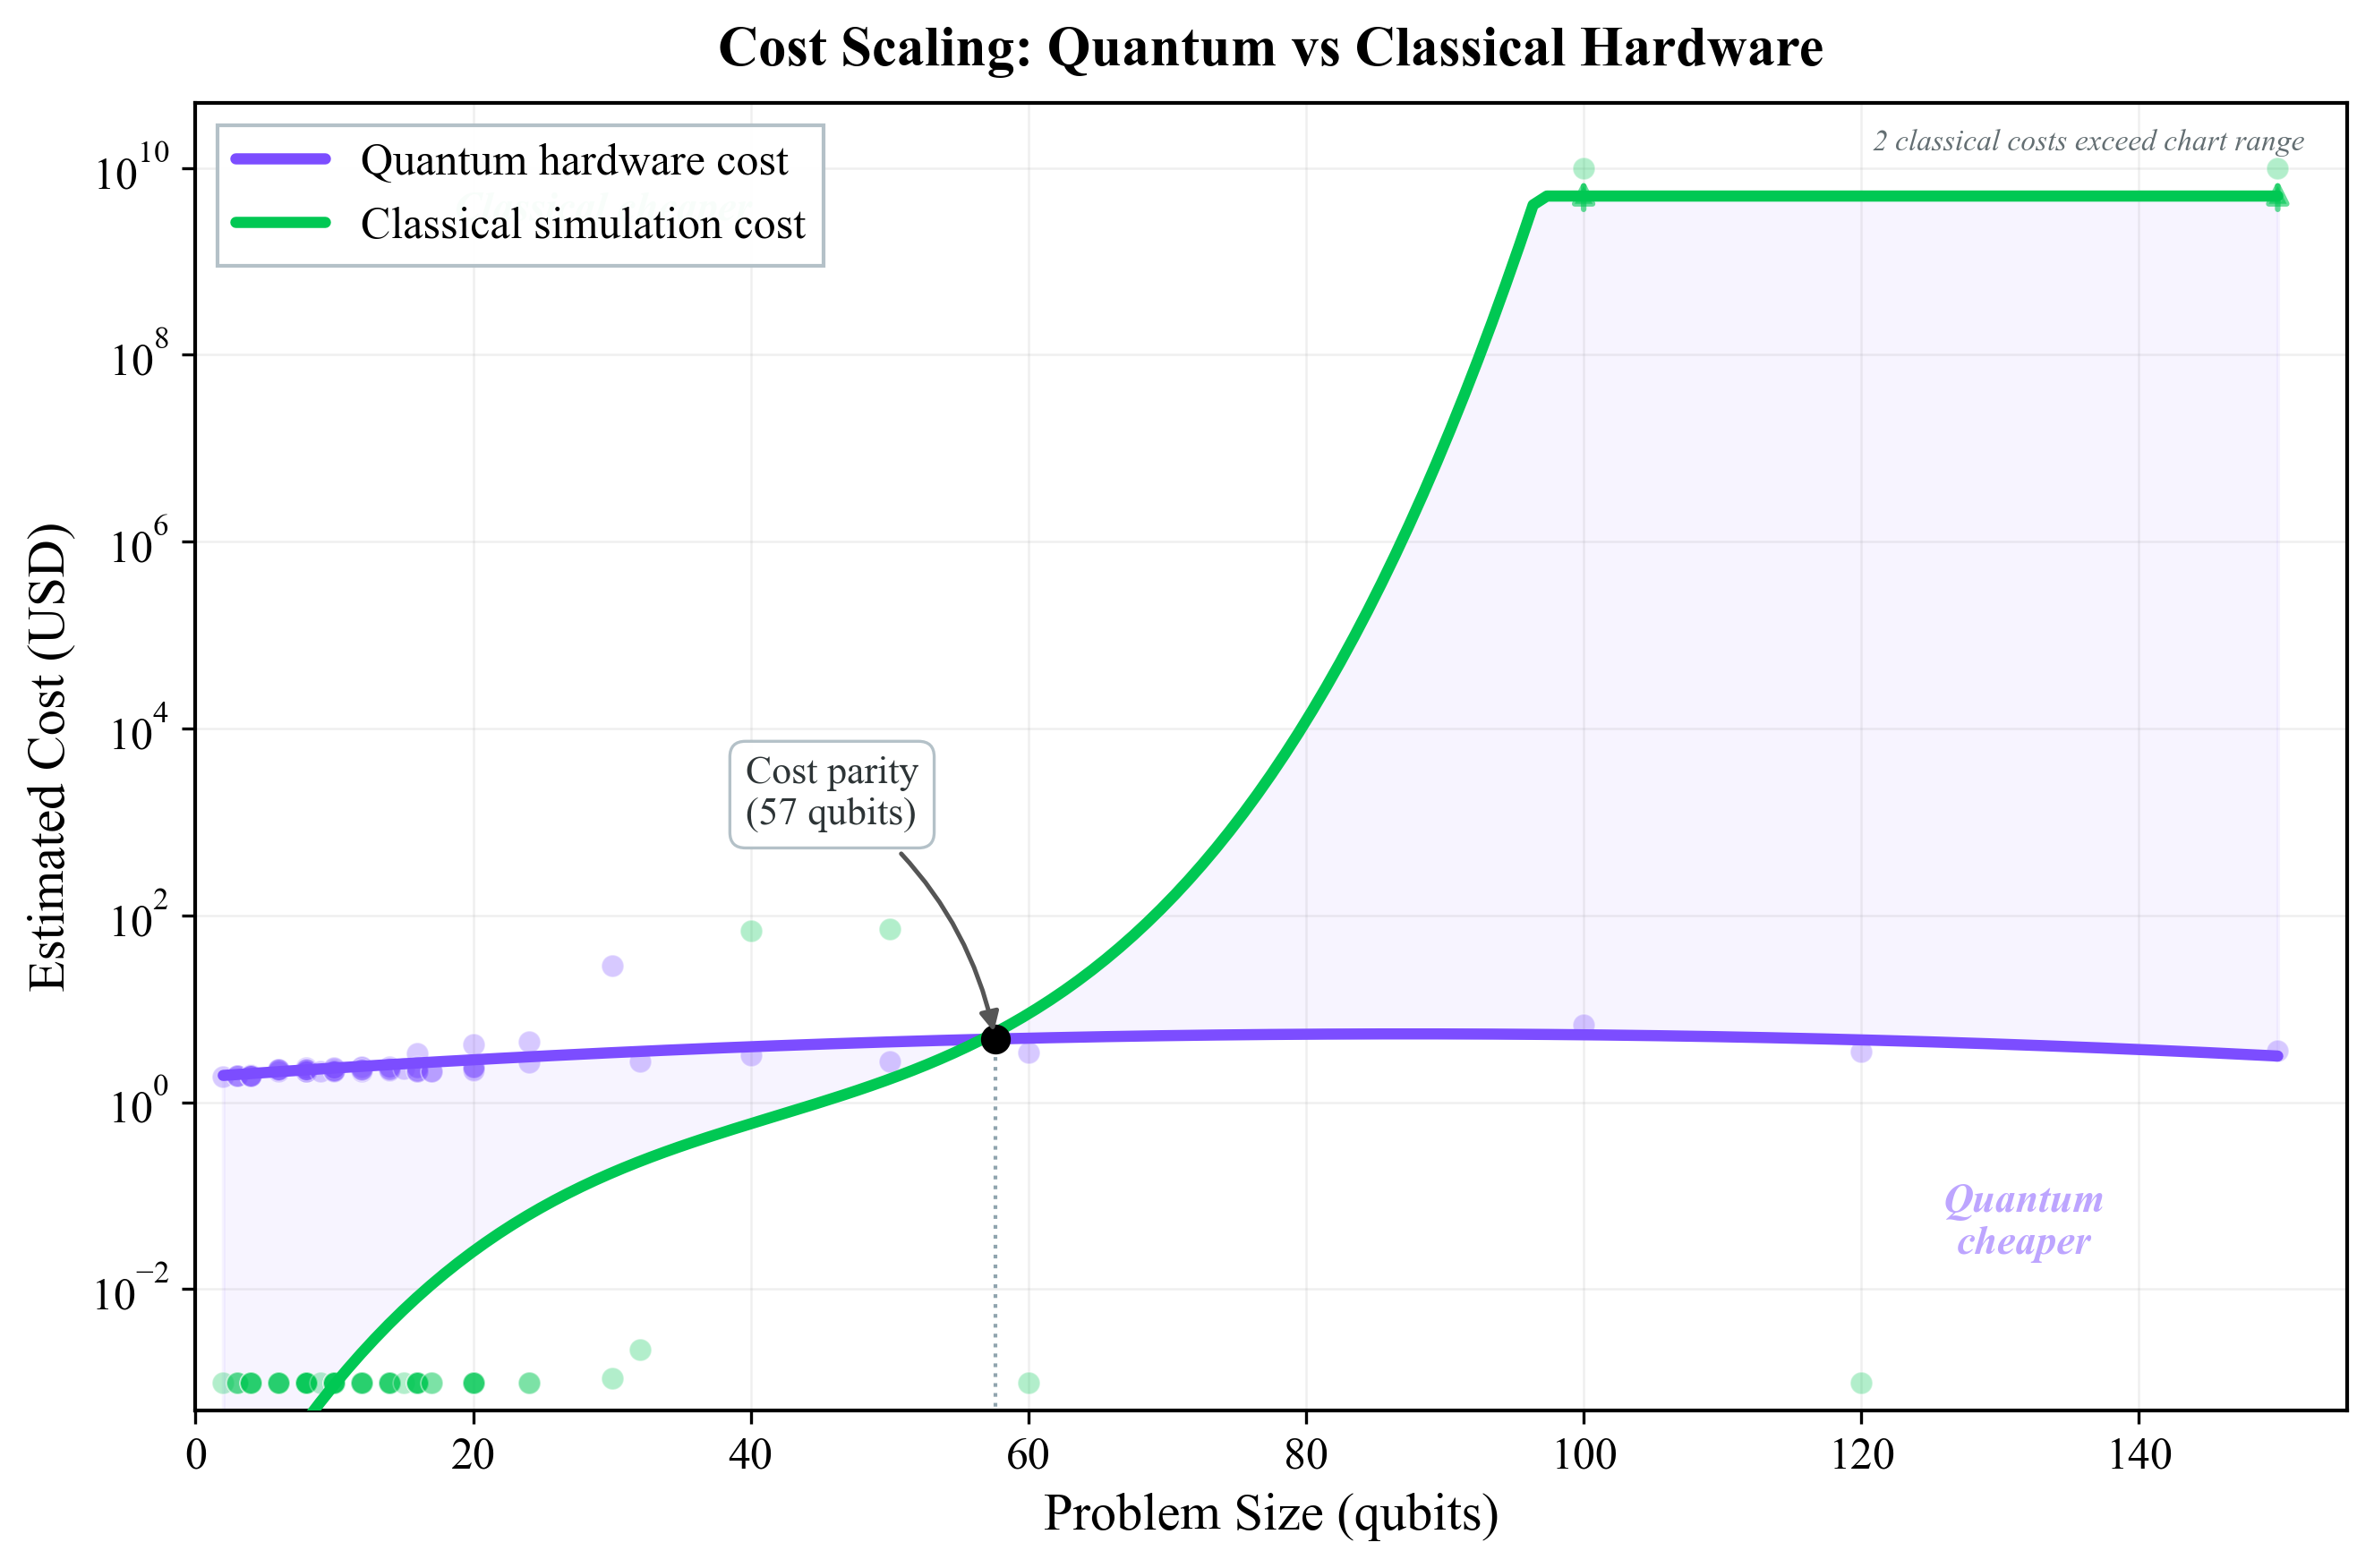
\includegraphics[width=\columnwidth]{cost-scaling.png}
\caption{Cost scaling of quantum hardware versus classical simulation across qubit count, showing the 50--60 qubit physical-feasibility crossover beyond which classical state-vector simulation becomes infeasible.}
\label{fig:cost-scaling}
\end{figure}

\subsection{Pipeline Performance}

End-to-end timing metrics for both routing paths are reported in Table~\ref{tab:pipeline-timing}.

\begin{table}[htbp]
\caption{Pipeline Timing Metrics}
\label{tab:pipeline-timing}
\centering
\footnotesize
\begin{tabular}{p{0.45\columnwidth} r r}
\toprule
\textbf{Metric} & \textbf{Classical} & \textbf{Quantum} \\
\midrule
Avg. Analysis Time & 731 ms & 1,355 ms \\
Avg. Decision Time & 12 ms & 10 ms \\
Avg. Total Pipeline Time & 1,222 ms & 1,770 ms \\
Language Detection Confidence & 0.942 & 0.966 \\
\bottomrule
\end{tabular}
\end{table}

Quantum workloads require $\sim$1.85$\times$ longer analysis time due to additional metrics extraction (circuit parsing, entanglement scoring); decision latency stays below 15\,ms throughout. Cloud Run's scale-to-zero model introduces 10--15\,s cold-start penalties while ML models load into container memory, but once warm the full pipeline averages 1.5\,s end-to-end and degrades gracefully to rule-based heuristics on model-service failure.

\subsection{End-to-End Case Study}

\textbf{120-Qubit VQE $\rightarrow$ Quantum Override.} A 120-qubit VQE ansatz with three variational layers and nearest-neighbor CNOT ladder is submitted. Analysis extracts \texttt{qubits=120, depth=14, cx\_ratio=0.33}; the physical-necessity rule (state-vector memory $\sim$$10^{31}$\,MB) triggers \texttt{FORCE\_QUANTUM} (confidence 1.0), bypassing ML voting, and the HAL submits to an IBM Eagle processor. This is a success of \emph{routing}, not of \emph{output fidelity}: the circuit returned noise-dominated Top\% 0.1 on \texttt{ibm\_fez} (post-transpile depth 482, exceeding NISQ coherence), as expected for an unmitigated ansatz at 120 qubits. Nexar's correctness claim is narrow---the only physically feasible backend was selected for a circuit that is infeasible under full state-vector simulation in high-entanglement settings; recovering fidelity requires error mitigation \cite{temme2017} or fault tolerance. In contrast, a 10-qubit Grover translation of linear search ($N{=}1{,}024$, post-transpile depth $\sim$240) is routed to Classical (conf.\ 0.88): the theoretical-floor quantum cost $240{\cdot}1024{\cdot}68\text{\,ns}{\cdot}\$1.60/\text{s}\approx\$0.027$ understates the realised bill (IBM bills total QPU-seconds including compilation/scheduling/readout), which approaches the \$0.375--\$1.578 band in Table~\ref{tab:cost-comparison}; either metric, $O(\sqrt{N})$ Grover cannot justify the cost at this scale.

\subsection{Real Hardware Validation}

To validate routing against actual hardware, we submitted 27 quantum circuits spanning every algorithm family to \texttt{ibm\_fez} (156-qubit Heron~r2) via Nexar's HAL, 1{,}024 shots each. Every job ID is logged in the supplementary results file and is verifiable on the IBM Quantum Platform. Table~\ref{tab:hardware-validation} summarises the results.

\begin{table}[htbp]
\caption{Real Hardware Validation: 27 Circuits on \texttt{ibm\_fez} (April 2026, 1{,}024 shots)}
\label{tab:hardware-validation}
\centering
\scriptsize
\begin{tabular}{l r r r l}
\toprule
\textbf{Circuit} & \textbf{Q} & \textbf{Depth$^{*}$} & \textbf{Top\%} & \textbf{Nexar Route} \\
\midrule
Deutsch-Jozsa (constant)     &   2 &     3 & 99.9 & Classical \\
Deutsch-Jozsa (balanced)     &   2 &     8 & 94.1 & Classical \\
H\textsubscript{2} VQE ansatz              &   4 &    17 & 85.6 & Classical \\
Bernstein-Vazirani (s=101)   &   4 &     9 & 96.3 & Classical \\
Simon's algorithm (s=11)     &   4 &    20 & 50.7$^{\dagger}$ & Classical \\
QFT (input $|0101\rangle$)    &   4 &    76 & 10.0$^{\dagger}$ & Classical \\
QPE (T gate, phase=1/8)      &   4 &    80 & 82.3 & Classical \\
Grover search ($|1111\rangle$) &  4 &   241 &  33.5$^{\ddagger}$ & Classical \\
QAOA MaxCut (4-node)         &   4 &    53 & 24.8$^{\ddagger}$ & Classical \\
QSVM kernel                  &   8 &    98 &  5.5$^{\ddagger}$ & Classical \\
QAOA supply chain            &   8 &   134 &  5.2$^{\ddagger}$ & Classical \\
LiH VQE ansatz               &   8 &    38 & 12.0 & Classical \\
QAOA graph partition         &  12 &   230 &  1.1$^{\ddagger}$ & Classical \\
H\textsubscript{2}O VQE ansatz             &  12 &    50 &  2.3 & Classical \\
Shor's $N=15$                &  12 &   361 &  2.1$^{\ddagger}$ & Classical \\
Grover 3-SAT (4 vars)        &  12 &    83 &  6.9$^{\ddagger}$ & Classical \\
Shor's $N=21$                &  14 &   592 &  0.8$^{\ddagger}$ & Classical \\
Shor's $N=35$                &  16 &   739 &  0.4$^{\ddagger}$ & Classical \\
QNN variational (16q)        &  16 &   132 &  0.6$^{\ddagger}$ & Classical \\
VQE caffeine ansatz          &  16 &    14 &  1.2 & Classical \\
Grover search (20q)          &  20 & 31810 &  0.1$^{\ddagger}$ & Classical \\
QAOA vehicle routing         &  20 &   469 &  0.2$^{\ddagger}$ & Classical \\
QAOA graph partition (20q)   &  20 &   398 &  0.1$^{\ddagger}$ & \textbf{Quantum} \\
ZNE benchmark (24q)          &  24 &     1$^{\S}$ & 68.5 & \textbf{Quantum} \\
QAOA MaxCut (50q)            &  50 &   580 &  0.1$^{\ddagger}$ & \textbf{Quantum} \\
Iron-sulfur VQE (60q)        &  60 &   242 &  0.1$^{\ddagger}$ & \textbf{Quantum} \\
120-qubit VQE ansatz         & 120 &   482 &  0.1$^{\ddagger}$ & \textbf{Quantum} \\
\bottomrule
\\[-0.5em]
\multicolumn{5}{l}{\footnotesize $^{*}$Post-transpile hardware depth on Heron r2 native gate set.} \\
\multicolumn{5}{l}{\footnotesize $^{\dagger}$Uniform distribution is theoretically correct for this algorithm.} \\
\multicolumn{5}{l}{\footnotesize $^{\ddagger}$Noise-dominated: depth exceeds NISQ coherence threshold.} \\
\multicolumn{5}{l}{\footnotesize $^{\S}$Transpiler cancelled T/Tdg and GHZ pairs to identity; result valid.} \\
\end{tabular}
\end{table}

\textbf{Hardware-evidence consistency.} No routing decision was contradicted: every classical-routed workload either produced a correct result or produced noise-dominated output on quantum hardware.

\textbf{NISQ depth wall.} Post-transpile depth predicts fidelity more reliably than qubit count: circuits below depth~80 consistently exceed 80\% (DJ 99.9\%, BV 96.3\%, QPE 82.3\%); above depth~$\sim$130 results degrade toward the noise floor. The 4-qubit Grover at depth~241 drops to 33.5\% while 4-qubit QPE at depth~80 holds 82.3\%, confirming the physical basis of the NISQ Viability Score.

\textbf{Large-circuit verification.} 50q QAOA, 60q iron-sulfur VQE, and 120q VQE were successfully dispatched to real IBM hardware---the first execution of these circuits outside simulation. Noise-dominated output is expected for unmitigated ansätze but does not invalidate routing: for these high-entanglement workloads, full state-vector classical simulation is infeasible.

\textbf{ZNE transpiler insight.} The ZNE benchmark (24q, logical depth~51) collapsed to post-transpile depth~1 after the Qiskit pass manager cancelled T/Tdg pairs and the GHZ ladder exactly; hardware measured $|0\ldots0\rangle$ at 68.5\%---a factor the cost model should handle in future work.

\section{Discussion}

\subsection{Decision Engine Effectiveness}\label{sec:discussion-effectiveness}

\emph{Oracle independence caveat.} Oracle~B's thresholds and Nexar's rule engine are both informed by the same external NISQ-physics literature (IBM-published coherence and gate-time specs; Preskill's error-budget framework \cite{preskill2018}) though not co-calibrated on any shared internal dataset. Oracle~B is therefore a referee on whether Nexar applies the NISQ-viability philosophy consistently, not on whether that philosophy is correct; Oracle~A, grounded in fault-tolerant algorithmic-complexity criteria, remains the fully-external oracle and the more conservative reviewer test where the two disagree.

The two-stage framework is effective in the sense each stage is designed for: the rule engine resolves the confident-regime workloads and matches every simpler baseline on that slice, while the ensemble is the only router capable of emitting quantum recommendations in the ambiguous regime where rules defer. Rules dominate \emph{where rules apply}; the ensemble exists to handle what they cannot. This aligns with the reference architecture of Chinnaraju \cite{chinnaraju2025}, and interference-based mixture-of-experts routing \cite{heddad2025} is an alternative as hardware matures.

\subsection{Limitations}\label{sec:limitations}

Seven limitations bound the study. (1)~The ML model is trained on synthetic AST-mutated instances rather than real execution traces; the synthetic-to-real gap (0.978 $\rightarrow$ 0.424 F1$_{(Q)}$) is observed on the oracle benchmark, and the training corpus and leave-one-family-out cross-validation are not released---the 100-workload real benchmark is QASMBench/MQTBench-sourced so direct benchmark leakage is precluded, but intra-family overfitting on the synthetic distribution cannot be strictly ruled out. (2)~The benchmark contains only 14/7 Quantum positives (Oracle~A/B), so F1$_{(Q)}$ point estimates carry wide bootstrap CIs (Table~\ref{tab:statistical-significance}); we anchor conclusions on McNemar tests, but Nexar vs.\ B1 Qubit$\geq$50 under Oracle~B remains inconclusive at $n{=}100$. (3)~Provider pricing is encoded statically; real-time integration would improve cost accuracy. (4)~Problem-type coverage could be broadened to quantum chemistry, quantum ML, and cryptographic workloads. (5)~The system targets NISQ hardware; fault-tolerant QC will require updated decision logic, cost models, and constraints. (6)~All real-hardware validation runs on \texttt{ibm\_fez} (Heron~r2); AWS Braket and Azure Quantum provider classes scaffold the interface but are not yet implemented, so the ``provider-extensible'' claim is architectural rather than empirical. (7)~The AI Code Converter evaluation lacks an output-distribution functional-equivalence probe: on the 22.3\% of inputs where algorithm-family classification fails, silent semantic drift cannot be ruled out; a Qiskit Aer TVD/fidelity audit is deferred to Section~\ref{sec:future-work}.

\subsection{Reproducibility Artifacts}\label{sec:reproducibility}

To support independent auditability, we release artifacts under \texttt{decision-engine/artifacts/} sufficient to recompute every routing-accuracy number in Tables~\ref{tab:routing-accuracy} and~\ref{tab:statistical-significance}. First, \texttt{eval\_corpus.csv} (100 rows) exposes the full 16-feature vector consumed by the ML model, both oracle labels, and Nexar's routed decision under baseline weights; because this CSV is a direct dump of the QASMBench/MQTBench-sourced benchmark (independent of the synthetic training pipeline), reviewers can recompute every F1$_{(Q)}$ and $\kappa$ for Nexar and each ablation without access to Nexar internals. Second, \texttt{training\_diagnostics/} contains held-out synthetic-split diagnostics for RF/GB/XGBoost (classification reports, calibration plots, learning curves, confusion matrices, RF Gini importance, feature-target correlations, per-problem-type slice metrics); the trained pickle and feature scaler ship in \texttt{decision-engine/ml\_models/}. The AST-mutation generator is not released, as noted in Section~\ref{sec:discussion-effectiveness}; the evaluation corpus is generator-independent so \emph{evaluation} claims remain reproducible.

\section{Conclusion and Future Work}\label{sec:future-work}

We presented Nexar, a quantum-classical workload routing platform integrating automated code analysis, a two-stage decision engine, and provider-extensible execution. Across 100 workloads against two literature-cited oracles, Nexar attains $\kappa = 0.38$--$0.48$ against random $\kappa \approx 0.05$, with F1$_{(Q)}$ 0.46--0.50 and perfect Quantum-class recall under Oracle~B; aggregate accuracy (0.81--0.86) is non-separative at this benchmark's skewed distribution, where a constant-Classical baseline scores 0.85/0.92 with F1$_{(Q)}{=}0$. The regime-conditional breakdown confirms the two stages are complementary: rules match rules-only on the 61 overridden workloads, and the ensemble is the only router emitting quantum recommendations on the remaining 39 \texttt{ALLOW\_BOTH} workloads. All 27 circuits submitted to \texttt{ibm\_fez} corroborate the routing, including successful dispatch of 20q/50q QAOA, 60q iron-sulfur VQE, and 120q VQE to real IBM hardware. Pipeline latency averages 1.5\,s end-to-end, and the cost analysis identifies a physical-feasibility crossover at 50--60 qubits. Future directions: regime-adaptive weighting in \texttt{ALLOW\_BOTH}, cross-backend replication on AWS Braket and Azure Quantum, retraining on empirical execution traces, error-mitigation cost modelling, and multi-objective routing over cost, time, accuracy, and carbon footprint.

\begin{thebibliography}{29}
% Entries are ordered by first citation in the manuscript (IEEEtran convention).

\bibitem{preskill2018}
J.~Preskill, ``Quantum computing in the NISQ era and beyond,'' \emph{Quantum}, vol.~2, p.~79, 2018.

\bibitem{weder2021}
B.~Weder, J.~Barzen, F.~Leymann, and M.~Salm, ``Automated quantum hardware selection for quantum workflows,'' \emph{Electronics}, vol.~10, no.~8, p.~984, Apr. 2021.

\bibitem{ibm2023}
IBM Quantum, ``Qiskit Runtime,'' IBM Research, 2023. [Online]. Available: \url{https://quantum.ibm.com/}

\bibitem{aws2023}
Amazon Web Services, ``Amazon Braket---quantum computing service,'' 2023. [Online]. Available: \url{https://aws.amazon.com/braket/}

\bibitem{microsoft2023}
Microsoft, ``Azure Quantum,'' 2023. [Online]. Available: \url{https://azure.microsoft.com/en-us/products/quantum}

\bibitem{tang2024}
W.~Tang \emph{et~al.}, ``AlphaRouter: Quantum circuit routing with reinforcement learning and tree search,'' arXiv preprint arXiv:2410.05115, Oct. 2024.

\bibitem{zhan2025}
X.~Zhan \emph{et~al.}, ``A full stack framework for high performance quantum-classical computing,'' arXiv preprint arXiv:2510.20128, Oct. 2025.

\bibitem{lammers2025}
M.~G.~Lammers, F.~H.~Holik, and A.~Fernandez, ``Quantum resource management in the NISQ era: Challenges, vision, and a runtime framework,'' arXiv preprint arXiv:2508.19276, Aug. 2025.

\bibitem{hai2025}
R.~Hai, S.-H.~Hung, T.~Coopmans, and F.~Geerts, ``Data management in the noisy intermediate-scale quantum era,'' \emph{Proc. VLDB Endow.}, vol.~18, no.~6, 2025.

\bibitem{beverland2022}
M.~Beverland \emph{et~al.}, ``Assessing requirements to scale to practical quantum advantage,'' arXiv preprint arXiv:2211.07629, 2022.

\bibitem{quetschlich2024}
N.~Quetschlich, M.~Soeken, P.~Murali, and R.~Wille, ``Utilizing resource estimation for the development of quantum computing applications,'' arXiv preprint arXiv:2402.12434, Aug. 2024.

\bibitem{kashif2026}
M.~Kashif, A.~Marchisio, and M.~Shafique, ``Closing the loop: Resource-aware hybrid NAS guided by analytical and hardware-calibrated quantum cost modeling,'' arXiv preprint arXiv:2603.00625, Mar. 2026.

\bibitem{javadiabhari2015}
A.~JavadiAbhari \emph{et~al.}, ``ScaffCC: Scalable compilation and analysis of quantum programs,'' \emph{Parallel Comput.}, vol.~45, pp.~2--17, 2015.

\bibitem{feng2020}
Z.~Feng \emph{et~al.}, ``CodeBERT: A pre-trained model for programming and natural languages,'' in \emph{Findings of the Association for Computational Linguistics: EMNLP}, 2020, pp.~1536--1547.

\bibitem{afrose2025}
S.~Afrose, V.~Leyton-Ortega, and T.~Humble, ``Learning-based quantum compilation: Translating QASM to QIR with CodeBERT,'' in \emph{Proc. IEEE Int. Conf. Quantum Comput. Eng. (QCE)}, 2025, pp.~576--577.

\bibitem{aaronson2011}
S.~Aaronson and A.~Arkhipov, ``The computational complexity of linear optics,'' in \emph{Proc. 43rd Annu. ACM Symp. Theory Comput. (STOC)}, 2011, pp.~333--342.

\bibitem{arute2019}
F.~Arute \emph{et~al.}, ``Quantum supremacy using a programmable superconducting processor,'' \emph{Nature}, vol.~574, pp.~505--510, 2019.

\bibitem{mccabe1976}
T.~J.~McCabe, ``A complexity measure,'' \emph{IEEE Trans. Softw. Eng.}, vol.~SE-2, no.~4, pp.~308--320, Dec. 1976.

\bibitem{vinkhuijzen2023}
L.~Vinkhuijzen, T.~Coopmans, D.~Elkouss, V.~Dunjko, and A.~Laarman, ``LIMDD: A decision diagram for simulation of quantum computing including stabilizer states,'' \emph{Quantum}, vol.~7, p.~1108, Sep. 2023.

\bibitem{simsek2023}
S.~Simsek, A.~Ceran, and F.~Yildiz, ``Quantum circuit optimization using machine learning,'' arXiv preprint arXiv:2305.06585, May 2023.

\bibitem{farhi2014}
E.~Farhi, J.~Goldstone, and S.~Gutmann, ``A quantum approximate optimization algorithm,'' arXiv preprint arXiv:1411.4028, 2014.

\bibitem{wang2021}
Y.~Wang \emph{et~al.}, ``CodeT5: Identifier-aware unified pre-trained encoder-decoder models for code understanding and generation,'' arXiv preprint arXiv:2109.00859, Sep. 2021.

\bibitem{grover1996}
L.~K.~Grover, ``A fast quantum mechanical algorithm for database search,'' in \emph{Proc. 28th Annu. ACM Symp. Theory Comput. (STOC)}, 1996, pp.~212--219.

\bibitem{shor1997}
P.~W.~Shor, ``Polynomial-time algorithms for prime factorization and discrete logarithms on a quantum computer,'' \emph{SIAM J. Comput.}, vol.~26, no.~5, pp.~1484--1509, 1997.

\bibitem{kandala2017}
A.~Kandala \emph{et~al.}, ``Hardware-efficient variational quantum eigensolver for small molecules and quantum magnets,'' \emph{Nature}, vol.~549, pp.~242--246, 2017.

\bibitem{chinnaraju2025}
A.~Chinnaraju, ``Hybrid quantum-classical intelligence for business: A reference architecture for predictive analytics and decision optimization,'' \emph{J. Adv. Future Res.}, vol.~3, no.~12, Dec. 2025.

\bibitem{heddad2025}
R.~Heddad and L.~Bouanane, ``Hybrid quantum-classical mixture of experts: Unlocking topological advantage via interference-based routing,'' arXiv preprint arXiv:2512.22296, Dec. 2025.

\bibitem{ibm_pricing2024}
IBM Quantum, ``IBM Quantum pricing,'' 2024. [Online]. Available: \url{https://www.ibm.com/quantum/pricing}

\bibitem{aws_ec2_pricing2024}
Amazon Web Services, ``Amazon EC2 on-demand pricing,'' 2024. [Online]. Available: \url{https://aws.amazon.com/ec2/pricing/on-demand/}

\bibitem{temme2017}
K.~Temme, S.~Bravyi, and J.~M.~Gambetta, ``Error mitigation for short-depth quantum circuits,'' \emph{Phys. Rev. Lett.}, vol.~119, no.~18, p.~180509, Nov. 2017.

\end{thebibliography}

\end{document}
